\lecture{22}{2025-05-07}{Méthode de Lagrange}{}
\subsubsection{Rappel Extrema liés. Méthode des multiplicateur de Lagrange}

\begin{parag}{Théorème (cas $n = 2$)}
    \begin{theoreme}
        Condition nécessaire pour un extremum sans contrainte.(mais qui n'est pas suffisante)\\
        Soit les fonctions $f, g: E^{\subset \mathbb{R}^2} \to \mathbb{R}$ de classe $C^1$.\\
        Supposons que $f\left(x, y\right)$ admet un extremum en $\left(a, b\right) \in E$ sous la contrainte $g\left(x, y\right) = 0$, Ce qui se dit tel que:
        un extremum de $\left\{f\left(x,y\right): \left(x, y\right) \in E \text{ et } g\left(x, y\right) = 0\right\}$. Et que $\nabla g\left(a, b\right) \neq \overline{0}$. \\
        Alors il existe $\lambda \in \mathbb{R}$ tel que:
        \begin{align*} 
            \nabla f\left(a, b\right) = \lambda \nabla g\left(a, b\right)
        \end{align*}
    \end{theoreme}
    
    \begin{definition}
        $\lambda$ est le multiplicateur de Lagrange
    \end{definition}
\end{parag}
\begin{parag}{Extrema liés: interpretation géométrique}
    soit $g\left(x, y\right) = 0 $ avec la contrainte que c'est sur une courbe de niveau, alors $\nabla g\left(x, y\right) \perp $ à cette courbe de niveau, $\nabla g\left(x, y\right) \neq \overline{0}$ (contrainte mentionnée dans le théorème).\\
    Si $\left(a, b\right)$ est un extremum local de $f\left(x, y\right)$ sur la courbe, il y a deux possibilités:
    \begin{itemize}
        \item Soit c'est un extremum local de $f$ sur $\mathbb{R}^{2}$
        \item Soit ce n'est pas un extremum local de de $f$ sur $\mathbb{R}^{2}$ mais un extremum local seulement sur la courbe.
    \end{itemize}
    Ce qui implique donc dans chaque cas:
    \begin{itemize}
        \item $\nabla f\left(a, b\right) = 0$
        \item $\nabla f\left(a, b\right) \perp$ à la courbe de niveau.
    \end{itemize}
    Ce qui implique donc que:
    \begin{itemize}
        \item $\nabla f\left(a, b\right) = 0 \cdot \nabla g\left(a, b\right)$
        \item $\nabla f\left(a, b\right) =  \lambda \cdot  \nabla g\left(a, b\right)$ où $\lambda \neq 0$
    \end{itemize}
    
\end{parag}

\begin{parag}{Démonstration}
    Pour la démonstration je renvoie le pdf de Joachim Favre qui est plus propre et plus clair que moi \\
Les idées majeurs sont TFI, qui permet de mieux réecrire notre fonction, par la suite la dérivée de la composition (avec la jacobienne avec le ``changement de variable''  :)
\begin{align*} \begin{pmatrix} 1 \\h\left(x\right)  \end{pmatrix}  \end{align*}



\end{parag}

\begin{parag}{Extrema liés cas général}
    \begin{theoreme}
        Soit $f, g_1, \ldots, g_m : E^{ \subset \mathbb{R}^{n}} \to \mathbb{R}$ les fonctions de classe $C^1$ tel que $m \leq n - 1$. Soit $\overline{a} \in E $ un extremum de $f$ sous les contraintes $g_1\left(\overline{x}\right) = \ldots = g_m\left(\overline{x}\right) = 0$.\\
        Supposons que les vecteurs $\nabla g_1\left(\overline{a}\right), \ldots, \nabla g_m\left(\overline{a}\right)$ sont linéairement indépendants.\\
        Alors il existe un vecteur $\overline{\lambda} = \left(\lambda_1, \ldots, \lambda_m\right) \in \mathbb{R}^{m}$ tel que:
        \begin{formule}
            \begin{align*} \nabla f\left(\overline{a}\right) = \sum_{k = 1}^{m} \lambda_k \nabla g_k\left(\overline{a}\right) \end{align*}
        \end{formule}
        
    \end{theoreme}
    Ici on utilise linéairement indépendant comme ``analogie'' à $\nabla g\left(a, b\right) \neq \overline{0}$ lorsque on avait $g: \mathbb{R}^{n} \to \mathbb{R}$. (maintenant on va dans $\mathbb{R}^{n}$)
    En particulier si on cherche un extremum de $f$ sour la contrainte $g\left(\overline{x}\right) = 0$ on obtient les équations:
    \begin{align*} 
        \begin{cases}
            \nabla f\left(\overline{x}\right) =  \nabla g\left(\overline{x}\right)\; \; \; \text{ si } \nabla g\left(\overline{x}\right) \neq 0 \text{ pour } g\left(\overline{x}\right) = 0\\
            g\left(\overline{x}\right) = 0
        \end{cases}
    \end{align*}
\end{parag}
\begin{parag}{Exemple 1}
    Trouver les extrema de la fonction $f\left(x, y, z\right) = 4x + 2y - z$ sous la contrainte $g\left(x, y, z\right) = x^2 + y^2 + z^2 - 21 = 0$ (qui est donc une sphère de rayon $\sqrt{21}$).\\
    On commence avec le théorème, le gradient: $\nabla g\left(2x, 2y, 2z\right) \neq \left(0, 0, 0\right)$ sur la sphère de rayon $\sqrt{21}$\\
    Alors, par le théorème de Lagrange, si on a $\left(x, y, z\right) \in $ sphère qui est un point d'extremum local de $f$ sur la sphère, alors, $\exists \lambda \in \mathbb{R}$ tel que:
    \begin{align*} 
        \nabla f\left(x, y, z\right) = \lambda \nabla g\left(x, y, z\right)\\
        x^2 + y^2 + z'2 =  21
    \end{align*}
    On a donc ici quatre équation dont les trois du gradients:
    \begin{align*}
        \begin{case}
            \left(4, 2, -1\right) =  \lambda \left(2x, 2y, 2z\right)\\
            x^2 + y^2 + z^2 =  21
        \end{case}
    \end{align*}
    Donc si on pose notre première trois relations:
    \begin{align*}
        \begin{case}
            4 =  \lambda 2x\\
            2 =  \lambda 2y \\
            -1 =  \lambda 2z
            \end{case} \implies \begin{case}
            x =  \frac{2}{\lambda}\\
            y =  \frac{1}{\lambda}\\
            z =  - \frac{1}{2\lambda}
        \end{case}
        \implies \begin{case} x =  -4z \\ y =  -2z \end{case}
    \end{align*}
    Et cela dans $g\left(x, y, z\right) =  0$.\\
    On implique ce qu'on trouve à notre contrainte:
    \begin{align*} 16z^2 + 4z^2 + z^2 =  21 \implies 21z^2 =  21 \implies z = \pm 1 \end{align*}
    Ce qui nous implique que: $z =  -1, y = 2, x = 4$ ou alors l'opposé qui nous donne:
    \begin{align*} \left(-4, -2, 1\right), \; \; \left(4, 2, -1\right) \end{align*}
    On remet notre valeur dans notre fonction:
    \begin{align*} f\left(-4, -2, 1\right) =  4x + 2y - z =  -16 -4 -1 =  -21\\
                    f\left(4, 2, -1\right) =  16 + 4 + 1 =  21
    \end{align*}
    Néanmoins ici on parle d'une sphère qui est un espace fermé dans $\mathbb{R}^{3}$, qui est aussi borné. Comme on est donc dans un ensemble compact, et puisque que notre fonction est aussi continue sur cette ensemble alors, notre fonction atteint \important{forcement} son maximum et son minimum sur la sphère.\\
    Ce qui implique que $f$ atteint son minimum et son maximum absolus sur la sphère.\\
    On va donc chercher les plans où il y a le minimum et le maximum, logiquement ces plans se retrouvent au sommets de la sphère, ces plans sont donc tangent à cette sphères:
    \begin{center}
        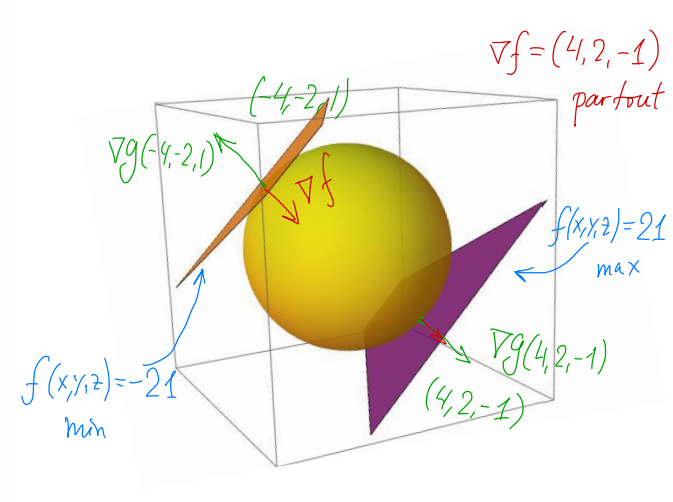
\includegraphics[scale=0.5]{12025-05-07.png}
    \end{center}
    Ici on a des plans qui sont en pente car on a notre plan  qui est ``pas tout joli'' ces plan veulent dire que notre fonction a toujours la même valeur dans ce point, et donc notre valeur a toujours la même valeur sur ce plan ce qui ``fausse'' notre idée d'un plan horizontale
    
\end{parag}
\begin{parag}{Example 2}
    Trouver les extrema de la fonction $f\left(x, y, z\right) =  xyz$ sous les contraintes 
    \begin{align*} \begin{cases}
        g_1\left(x, y, z\right) = x + y + z - 5 =  0\\
        g_2\left(x, y, z\right) =  xy + yz + xz - 8 =  0
    \end{cases} \end{align*}
    On va donc chercher:
    \begin{align*} \nabla g_1 \left(x, y, z\right) =  \left(1, 1, 1\right) \forall \left(x, y, z\right) \in \mathbb{R}^{3}\; \; \; \; \nabla g_2 \left(x, y, z\right) =  \left(y + z , x + z, x + y\right) \; \forall \left(x, y, z\right) \in \mathbb{R}^{3} \end{align*}
    On va donc chercher:
    \begin{align*} \nabla g_2\left(x, y, z\right) =  k \nabla g_1\left(x, y, z\right) \implies \left(y + z, x + z, x + y\right) = \left(k, k, k\right) \implies x =  y = z \end{align*}
    Et donc si on remplace ce que l'on vient de trouver dans notre fonction $g$:
    \begin{align*} 
        \begin{case}
            g_1\left(x, x, x\right) =  3x - 5 = 0 \implies x =  \frac{5}{3}\\
            g_2\left(x, x, x\right) =  3x^2 - 8 = 0 \implies 3\left(\frac{5}{3}\right)^2 =  \frac{25}{3} \neq 8
        \end{case}
    \end{align*}
    Ce qui implique donc que $\nabla g_1\left(x, y, z\right)$ et $\nabla g_2\left(x, y, z\right)$ sont linéairement indépendants ce qui implique que le théorème de Lagrange est applicable.\\
    Et donc obtient donc les équations:
\begin{align*}
    \begin{case}
        \nabla f\left(x, y, z\right) =  \left(yz, xz, xy\right) =  \lambda_1\left(1, 1, 1\right) + \lambda_2 \left(y + z, x + z, x + y\right)\\
        g_1\left(x, y, z\right) =  x + y + z - 5 =  0\\
        g_2\left(x, y, z\right) =  xy + yz + xz - 8 = 0
    \end{case}
\end{align*}
Ce qui nous donne:
\begin{align*} 
    \begin{case}
        yz =  \lambda_1 + \lambda_2 \left(y + z\right)\\
        xz =  \lambda_1 + \lambda_2\left(x + z\right)\\
        xy =  \lambda_1 + \lambda_2\left(x + y\right)\\
        x + y + z = 5\\
        xy + yz + xz =  8
    \end{case}
\end{align*}
Donc on voit ici que ça a l'air embêtant à faire donc on va se poser quelque minute pour voir s'il y a quelque chose afin d'accélérer tout ça.\\
Si on additionne nos deux première relations: 
\begin{align*} \left(1\right) + \left(2\right) \implies z\left(x + y\right) =  2\lambda_1 + \lambda_2\left(x + y + 2z\right)\\
    z\left(5-z\right) =  2\lambda_1 + \lambda_2\left(5 + z\right)
\end{align*}
On obtient donc une équation quadratique pour $z$.\\
Si on additionne $\left(2\right) + \left(3\right)$:
\begin{align*} x\left(5-x\right) =  2\lambda_1 + \lambda_2\left(5 + x\right) \end{align*}
Et finalement pour $\left(1\right) + \left(3\right)$:
\begin{align*} y\left(5-y\right) = 2\lambda_1 + \lambda_2\left(5 + y\right) \end{align*}
Ce qui revient donc:
\begin{align*} 
    \begin{case}
        z^2 + \left(\lambda_2 - 5\right)z + 5\lambda_2 + 2\lambda_1 =  0\\
        x^2 + \left(\lambda_2 - 5\right)x + 5\lambda_2 + 2\lambda_1 = 0\\
        y^2 + \left(\lambda_2 - 5\right) y + 5\lambda_2 + 2\lambda_1 = 0
    \end{case}
\end{align*}
Vu qu'on a trois fois la même équations; soit $x= y= z$ qui ne satisfait pas les contraintes, soit une variable différente des $2$ autres, par exemple $x =  y, z \neq x$.\\
On peut maintenant utiliser les équations (4) et (5):
\begin{align*} 
    \begin{case}
        2x + z =  5\\
        x^2 + 2xz =  8
        \end{case} \implies \begin{case} z = 5 - 2x\\ x^2 + 2x\left(5-2x\right) - 8 =  0 \implies 3x^2 + 10x - 8 = 0\end{case}
\end{align*}
Donc on peut résoudre notre équation tel que:

\begin{align*} 
    x = \frac{10 \pm \sqrt{100 - 96}}{6} =  \frac{10 \pm 2}{6} \\
    \implies x_1 =  2 =  y_1 \implies z_1 =  1\\
    \implies x_2 =  \frac{4}{3} =  y_2 \implies z_2 =  \frac{7}{3}
\end{align*}
Donc ici les points qu'on a trouvé sont:
\begin{align*} \left(x, y, z\right) =  \left(2, 2, 1\right), \left(1, 2, 2\right), \left(2, 1, 2\right)\\
\left(\frac{4}{3}, \frac{4}{3}, \frac{7}{3}\right), \left(\frac{7}{3}, \frac{4}{3}, \frac{4}{3}\right), \left(\frac{4}{3}, \frac{7}{3}, \frac{4}{3}\right)\end{align*}
Qui sont donc nos 6 points candidats. Donc il suffit maintenant de trouver on faisant les calculs:
\begin{align*} 
    f\left(2, 2, 1\right) =  f\left(1, 2, 2\right) =  f\left(2, 1, 2\right) =  4\\
f\left(\frac{4}{3}, \frac{4}{3}, \frac{7}{3}\right) = f\left(\frac{7}{3}, \frac{4}{3}, \frac{4}{3}\right) =f \left(\frac{4}{3}, \frac{7}{3}, \frac{4}{3}\right) = \frac{112}{3}
\end{align*}
Puisque les $g_1\left(x, y, z\right) =  0$, $g_2\left(x, y, z\right)$ est compact dans $\mathbb{R}^{3}$ et $f$ est continue. Alors $f$ atteint son min et son max sur le  compact; $f$ est de classe $c^{\infty}$ alors $f$ atteint son max, min, aux points donnés par notre calcul.\\
\begin{subparag}{remarque}
    Ici il faudrait aussi prouver que le sous-ensemble soit compact
\end{subparag}

\end{parag}
\section{Résumé: Méthode de démonstration}
\begin{parag}{Démonstration direct}
   \begin{align*} P \implies Q \end{align*}
   A base de logique tel que:
   \begin{align*} P \implies \ldots \implies Q \end{align*}
\end{parag}
\begin{parag}{Par contraposée}
   \begin{align*} P \implies Q \end{align*} 
   On le prouve tel que :
   \begin{align*} \neg Q \implies \ldots \implies \neg P \end{align*}
\end{parag}
\begin{parag}{Disjonction des cas}
    \begin{align*} P \implies Q \end{align*}
    On le fait par cas:
    \begin{align*} 
        P = \begin{case}
            \text{cas 1} \implies Q\\
            \vdots\\
            \text{ cas n} \implies Q
        \end{case}
    \end{align*}
\end{parag}

\begin{parag}{Si et seulement si}
    \begin{align*} \iff \end{align*}
\end{parag}

\begin{parag}{Par récurrence}
   \begin{align*} P\left(n\right) \end{align*} 
   \begin{subparag}{Simple}
       \begin{itemize}
           \item \textbf{Base}: $P\left(n_0\right)$
           \item \textbf{Hérédité}: $P\left(n\right) \implies P\left(n+1\right)$
       \end{itemize}
   \end{subparag}
   \begin{subparag}{Généralisé}
       \begin{itemize}
           \item \textbf{Base}: $P\left(n_0\right), \ldots, P\left(n_0 + k\right)$
           \item \textbf{Hérédité}: $\left\{P\left(n\right), \ldots, P\left(n + k\right)\right\} \implies P\left(n+k+1\right)$
       \end{itemize}
   \end{subparag}
   \begin{subparag}{Forte}
       \begin{itemize}
           \item \textbf{Base}: $P\left(n_0\right)$
           \item \textbf{Hérédité}: 
       \end{itemize}
       
   \end{subparag}
\end{parag}











\begin{parag}{Exemple: choisir la méthode de démonstration}
    \begin{subparag}{Proposition 1}
        Pour tout $n \in \mathbb{N}$, $2n^2 + n + 1$ n'est pas divisible par $5$.
    \end{subparag}
    \begin{subparag}{Question 2}
        Il y a 12 boules vertess, $15$ boules rouges et 16 boules blanches dans un sac, Quel nombre minimal de boules faut-il sortir du sac pour avoir au moins $4$ boules de même couleur?
    \end{subparag}
    \begin{subparag}{Proposition 3}
            Il existe une infinité de nombre premier tels que:
            $p + 2$ n'est pas premier.
    \end{subparag}
    \begin{subparag}{Proposition 4}
        Il n'existe pas de nombre entiers $x, y$ tels que $42x - 70 y =  124$
    \end{subparag}
    \begin{subparag}{Proposition 5}
        Pour tout $n \geq 2$ naturel, on a:
        \begin{align*} P\left(n\right): \prod_{k = 2}^{n} \left(1- \frac{1}{k^2}\right)  \end{align*}
    \end{subparag}
    \begin{subparag}{Proposition 6}
        Si $f: \mathbb{R}^{3} \to \mathbb{R}$ de classe $C^2$, telle que $\det $ Hes$s_f\left(\overline{0}\right) < 0$, Alors $\overline{0}$ n'est pas un point de minimum local de $f$
    \end{subparag}
    \begin{subparag}{Proposition 7}
        Soient $x, y \in \mathbb{R}$. Si $y^3 + yx^2 - x^3 \leq xy^2$, alors $y \leq x$
    \end{subparag}
\end{parag}
\begin{parag}{Méthode}
    
    \begin{subparag}{Proposition 1}
        Pour cette méthode on va plutôt utilise la disjonction des cas comme la plupart des propositions avec la divisibilité
    \end{subparag}
    \begin{parag}{Question 2}
        Ici on utilise Les tiroirs car un a un nombre ``minimale'' qui peut facilement se compter.
    \end{parag}
    
    \begin{subparag}{Proposition 3}
        On utilise l'absurde avec le Euclide\\
        On prends un premier $q$ premier quelque part tel que $q + 2$ est premier néanmoins si on prends donc $q\left(q+2\right)$ est un nombre qui rentre dans la contradiction.
    \end{subparag}

    \begin{subparag}{Proposition 4}
        Donc ici on fait par l'absurde tel que ``imaginons que cela existe'' on voit que cela est une contradiction, donc cela ne peut pas exister.
    \end{subparag}
    \begin{subparag}{Proposition 5}
        
    \end{subparag}
    \begin{subparag}{Proposition 6}
        Ici on peut juste faire une preuve direct
    \end{subparag}
    \begin{subparag}{Proposition 7}
        Ici on utilise la contraposée 
    \end{subparag}
\end{parag}



\begin{parag}{Question}
    Soit une famille des propostions $\left\{P\left(n\right)\right\}_{n \in \mathbb{N}}$, telle que, pour tout $n \in \mathbb{N}$, si $P\left(n\right)$ est vraie, alors $P\left(n+4\right)$ est vraie.\\
    Alors:
    \begin{enumerate}
        \item $P\left(6\right)$ et $P\left(8\right)$ ne peuvent pas être vrai les deux
        \item si $P\left(19\right)$ est vrai, alors $P\left(7\right)$ est vraie
        \item $P\left(2\right)$ et $P\left(10\right)$ sont soit les deux vraies, soit les deux fausses
        \item si $P\left(21\right)$ est fausse, alors $P\left(9\right)$ est faux
    \end{enumerate}
    

\end{parag}

